\section{Problema 2}

\subsection{Resolución}

\subsubsection{Explicación del problema}
\indent El objetivo de este ejercicio es, dada un red de amistades y 2
investigadores, determinar cuántas veces el entusiasmo que se genera en uno de
ellos se verá fraccionado hasta, finalmente, generar un cierto entusiasmo en el
otro. \\
\indent Esto sucederá sólo en aquellos casos en los cuales estos investigadores
tengan amigos en común. En caso de existir varias redes de amistades
(entendiéndose por red de amistad a una conexión de amistades entre ambos
investigadores, sin que haya investigadores repetidos), se debe estudiar el caso
de la más corta, ya que esta red será la que generará el entusiasmo en el
investigador antes que cualquier otra y con la mayor proporción. \\
\indent Si no existiesen amigos en común entre ellos, es decir, si no existe una
red de amistad entre ambos, entonces el entusiasmo generado en uno nunca llegará
al otro, es decir la fracción de entusiasmo que le generará al investigador
destinatario será cero o, como se ha establecido, se indicará con $0$ la
cantidad de veces que éste se verá fraccionado.

\subsubsection{Primeros intentos de solución}
\indent En una primera aproximación al problema, pensamos en aplicar el
concepto de matrices de incidencia,
teniendo como índices a los investigadores por un lado y a las amistades por el
otro.\\
\indent Este clase de solución nos parecía productiva ya que al utilizar una
matriz, tanto para rellenarla en su totalidad como para recorrerla, los
algoritmos tienen una complejidad lineal O($m*n$), con $m$= cantidad de
amistades y $n$=cantidad de investigadores, quedando en evidencia que dicha
implementación cumplía la cota de complejidad pedida. \\
\indent Esta solución fue descartada una vez ya empezada su implementación.
Luego de buscar alguna estructura adecuada para representar a la matriz,
decidimos utilizar un diccionario de clave investigador y significado Lista de
amigos.\\
\indent El problema surgió a la hora de pensar un algoritmo para recorrer las
amistades con algún criterio y que no repita ninguna amistad. Luego de
contemplar varias opciones para tratar de solucionar este problema, nos dimos
cuenta de que estaba mal pensado el problema, ya que la matriz carecía de toda
la
información relevante necesaria para realizar el algoritmo del recorrido de la
misma. Incluso sabiendo qué amistad se había recorrido, era difícil establecer
un criterio de recorrido que nos diera el largo de la red de amistades más corta
que conecta a 2 investigadores (luego explicamos por qué nos interesa ésta red
en particular \footnote{ver Aplicación de BFS}.


\subsubsection{Aplicación de BFS al problema}
\indent \Obs{\textit{Estudiando los casos de tests provistos por la cátedra, 
pudimos observar que, cuando existen más de dos redes de amigos que conectan a
ambos investigadores,
el criterio para elegir una red de amigos, a través de la cuál 
se propaga el entusiasmo, es la que está conformada por la de menor cantidad de
investigadores.} }\\

\indent Antes que nada, realizamos el modelado del problema de esta forma:
Tomamos un grafo genérico $G(V,E)$, donde $V$ es el conjunto de vértices (y un
vértice es un 
investigador) de $G$ y $E$ un conjunto de pares de vértices(y un par de vértices
corresponde a la amistad entre
2 investigadores) , indicando las aristas que unen a dichos vértices en $G$.\\

\indent Dada una red de amigos, para saber cuántas veces se fracciona a la mitad
el entusiasmo del investigador $v_1$ hasta que recibe una porción de este el
investigador $v_n$, asumiendo que $v_1$ y $v_n$ tienen una red que los conecta,
tenemos la siguiente caracterización:
\begin{itemize}
 \item Si $v_1$ es amigo de $v_n$, entonces $v_n$ recibe la mitad del entusiasmo
de $v_1$, 
 ya que esta se divide a la mitad una sola vez y, a su vez, existe una única
arista en el camino que conecta a ambos.
 \item Si no son amigos, entonces cada uno de los amigos de $v_1$ reciben la
mitad del entusiasmo de $v_1$. Asumamos que $v_n$ se encuentra a distancia $n-1$
de $v_1$ y tomemos el único amigo de $v_1$, siendo este uno de los vértices del
camino mínimo que une a $v_1$ con $v_n$, al que llamaremos $v_2$. \\ 
\indent\indent Entre $v_1$ y $v_2$ hay una arista ($v_2$ se encuentra a
distancia 1 de $v_1$) y el entusiasmo de $v_1$ se fracciona una sola vez. Ahora,
entre $v_2$ y su amigo $v_3$, siendo este uno de los vértices del camino mínimo
que une a $v_1$ con $v_n$, entre $v_2$ y $v_3$ hay una arista ($v_3$ se
encuentra a distancia 1 de $v_2$). Entonces, entre $v_3$ y $v_1$ hay 2 aristas
($v_3$ se encuentra a distancia 2 de $v_1$) y el entusiasmo de $v_1$ se
fracciona una vez más que para $v_2$, es decir el entusiasmo de $v_1$ se
fracciona 2 veces hasta llegar a $v_3$. \\
\indent\indent Generalizando, para cualquier amigo $v_k$, con 2 $\leq$ k $\leq$
n:
 \begin{itemize}
  \item entre $v_k$ y $v_1$ hay k-1 aristas, es decir, se encuentran a distancia
k-1;
  \item el entusiasmo de $v_1$ se fracciona k-1 veces hasta llegar a $v_k$, y 
 \end{itemize}
\end{itemize}
\indent\indent Además, de existir otra red de amistades a través de la cual se
conectan ambos investigadores, pero cuya longitud es mayor o igual a la red en
cuestión, se desprecia el entusiasmo aportado por la otra, ya que el máximo del
entusiasmo original será aportado por la red de menor distancia. Es por esto que
siempre tenemos en cuenta sólo la red de amistades más corta
que une a ambos investigadores.\\

\indent Entonces, la cantidad de veces que se fracciona el entusiasmo de
$v_1$ hasta llegar a $v_n$ 
 es equivalente a la cantidad de aristas que exiten entre esos 2, es decir la
distancia entre ellos que es n-1.
 Es por esto que pudimos establecer la resolución del problema mediante
el uso del algortimo BFS, ya que la cantidad de fracciones que se produce sobre
el entusiasmo de $v_1$ hasta que genera algún nivel de entusiasmo en $v_n$, es
equivalente a calcular la distancia desde $v_1$ hasta $v_n$, que es lo que
calcula el BFS.\\

\indent Teóricamente, si la red de amigos en común más corta que
une $v_1$ con $v_n$ tiene un longitud $\delta$($i_1$,$v_n$) y $v_1$ se
entusiasma en un valor medible $e$,
luego $v_n$ se
entusiasmará con un nivel
\Gather{e' = \frac{e}{2.\delta(v_1,v_n)}.}

\indent Nuestra implementación trabaja con listas de adyacencia. Cada
investigador tiene asociada una lista donde están almacenados sus amigos (los
vértices adyacentes). Además, los investigadores poseen un campo estado que
puede tener alguno de los siguientes valores:

\begin{itemize}
\item \textit{no encontrado}: sería el equivalente al color blanco del algoritmo
de BFS, indicando que el recorrido del análisis de las amistades jamás abarcó
éste investigador. Inicialmente todos los investigadores están seteados
en este estado.
\item \textit{encontrado}: sería el equivalente al color gris del algoritmo de
BFS, indicando que ya se ha guardado este investigador en una cola para,
posteriormente, realizar el análisis sobre sus amistades.
\item \textit{visitado}: sería el equivalente al color negro del algoritmo de
BFS, indicando que ya se han guardado todos sus vértices adyacentes para su
análisis.
\end{itemize}

\hspace{-0.5cm}La función BFS realiza los siguientes pasos:
\begin{enumerate}
 \item Setea el estado del investigador fuente $s$ en gris.
 \item Encola $s$ en una cola vacía $c$.
 \item Desencola $c$ y ese elemento se almacena en $i$.
 \item Encola en $c$ los amigos de $i$.
 \item Setea el estado de $i$ en negro.
 \item Repite desde el paso 3 hasta que la cola quede vacía.
\end{enumerate}

\indent Una vez visitados todos los investigadores, se tiene como
postcondición que a todos se les ha seteado la distancia a $s$. En caso de que
no existiera un camino hacia $s$, la distancia por defecto no se modifica.\\ 
\indent El resultado de la función es el campo distancia del investigador
destinatario en caso de existir un camino entre él y $s$, o 0 en caso
contrario.\\
\indent Es importante notar que los investigadores se encolan y desencolan una
sola vez, ya que una vez encolados se los marca como ``encontrado", y una vez
desencolado se los marca como ``visitado", evitando así que en otra iteración se
los vuelva a encolar.

\subsubsection{Pseudocódigo}

\indent Para resolver el problema, utilizamos una función  llamada BFS
\footnote{Es una adaptación del modelo en: Cormen, Thomas... [et al];
\textit{Introduction to Algorithms}, Cambridge, MIT Press, 2009; (p\'ag. 595)}
, que toma
2 datos de tipo investigador. donde investigador es una clase que posee la
siguiente información sobre el investigador:
\begin{itemize}
	\item nombre
	\item estado (no encontrado, encontrado, visitado)
	\item lista de amistades directas
	\item distancia al vértice desde el cuál se quiere calcular la distancia
\end{itemize}
\indent La función que resuelve el problema propiamente dicho, se llama BFS, y
se encuentra dentro de la clase relaciones. Esta clase contiene:
\begin{itemize}
\item una lista de todos los investigadores.
\item un investigador fuente.
\item un investigador destino.
\end{itemize}

\begin{algorithm}
\caption{BFS (\textbf{in/out} source,destination: \textsl{Investigador})
$\rightarrow$ res: \textsl{int}}
\begin{algorithmic}[1]

\STATE $source.estado \leftarrow encontrado$
\STATE $source.distancia \leftarrow 0$
\STATE $cola \leftarrow \emptyset$
\STATE $encolar(cola,source)$
\WHILE{$cola \neq \emptyset$}
	\STATE $actual \leftarrow desencolar(cola)$
	\FORALL{$v \in amigos(actual)$}
		\IF{$v.estado == no encontrado$}
			\STATE $v.estado \leftarrow encontrado$
			\STATE $v.distancia \leftarrow actual.distancia + 1$
			\STATE $encolar(cola,v)$
		\ENDIF
	\ENDFOR
	\STATE $actual.estado \leftarrow visitado$
\ENDWHILE
\IF{$destination.distancia == \infty$}
	\RETURN $0$
\ELSE
	\RETURN $destination.distancia$
\ENDIF
\end{algorithmic}
\end{algorithm}

\subsection{Demostracion de correctitud}
\indent Dado que utilizamos el algoritmo de BFS y lo relacionamos con nuestro
problema, que nuestro codigo y pseudocodigo cumplen con el algoritmo, y que
utilizamos como bibliografia de consulta el libro ``Introduction to Algorithms''
de Thomas H. Cormen \& Cia., en el cual se encuentra explicada  explicitamente
dicha demostracion paso por paso en las páginas 599 y 600, no realizamos
correctitud del algoritmo de BFS.

\subsection{Complejidad}
\subsubsection{Análisis de complejidad}
\indent Analizamos el código de la función BFS línea por línea, siguiendo los
siguientes criterios:
\begin{itemize}
 \item Asignar valores enteros o chars acotados y comparar chars acotados
 tienen complejidad O(1). Los chars que comparamos son acotados por la
 longitud de ``no encontrado'' que es 13, ya que solo se
 comparan 3 strings posibles: ``encontrado'', ``visitado'' y ``no encontrado'',
y
 el más largo es este último
 \item Pedir alguna de las variables del tipo Investigador tiene una complejidad
$O(1)$, 
 ya que se puede acceder a estas directamente.
 \subitem La función constructora del tipo Investigador tiene una complejidad 
 O($|$nombre$|$) + O($|$estado$|$) + O(crear una lista vacia) + O(pedir max
value) =
 O(1) + O(1) + O(crear una lista vacia) + O(1) = O(crear una lista vacia)
 ya que los nombres de los investigadores y los strings que indican el estado
 son strings acotados por el más largo, que sabemos que será finito, por ende
toman O(1), y
 pedir el max value toma O(1)
 \item Las funciones del tipo genérico ``Queue''tienen la siguiente complejidad:
 \subitem crear una cola= O(crear lista enlazada)= O(1)
 \subitem ver si es vacía= O(1)
 \subitem encolar= O(1)
 \subitem desencolar= O(1)
 \item Las funciones del tipo genérico
``ArrayList''\footnote{http://docs.oracle.com/javase/6/docs/api/, java.utils,
ArrayList}  tienen
 la siguiente complejidad:
 \subitem crear iterador sobre ella = O(1)
 \subitem pedir el elemento de un índice= O(1)
 \subitem ver si hay siguiente= O(1)
 \subitem avanzar el iterador= O(1)
 
\end{itemize}

\indent Dado que estas son las únicas funciones que utilizamos en el código de
la función BFS, todas las líneas tienen complejidad O(1)\\
\indent Sólo falta analizar cuántas veces iteran los 2 whiles, para saber la 
complejidad de los mismos\\

%ESTO PARA ABAJO CAMBIA SI ALGUNA DE LAS FUNCIONES DENTRO DEL WHILE NO TOMA O(1)
\indent La complejidad del while más grande está determinada por la cantidad de
veces que itera 
y cada iteración toma O(cantidad de iteraciones del while anidado), es por esto
que
primero realizaremos el análisis del while anidado.\\

\indent El while anidado itera la lista de adyacencia de cada investigador $i$,
entonces
el while iterará $a_i$ veces, donde $a_i$ es el largo
de la lista de adyacencia de $i$.\\

\indent Ahora podemos determinar la complejidad del while más abarcativo. 

\indent Este ciclo iterará hasta que la cola $c$ quede vacía. $C$ es la cola
donde se irá guardando
sólo una vez los investigadores. Entonces esta cola no quedará vacía hasta que
se haya encolado y desencolado 
a todos los investigadores de ella. Por ende, este while itera tantas veces como
investigadores haya.\\

\indent Además, por cada iteración, este while toma una complejidad O($a_i$),
donde $a_i$ es el largo
de la lista de adyacencia de $i$, que es el
investigador que se ha desencola ni bien se entra en el while. Como este while
itera una vez para cada investigador,
la complejidad que tomará finalmente será 
\Gather{O(\sum_{i=1}^{k}(a_i+1)))} donde k es la cantidad de investigadores y se
suma uno para representar el costo adicional de cada iteración (que toma
O(1)).\\

Usando propiedades de sumatoria, nos queda que la complejidad es:
\Gather{O(\sum_{i=1}^{k}(a_i) + k) = O(\sum_{i=1}^{k}(a_i))+ O(k)}

\indent Observar que la sumatoria, representa a la suma del largo de la lista de
adyacencia de cada investigador, ya que en cada iteración del while se recorre
la lista de adyacencia de un investigador y esto se realiza una única vez para
todo investigador, entonces su resultado es 
\Gather{O(\sum_{i=1}^{k}(a_i))= O(2a)}
siendo $a$ la cantidad de amistades total. Esto se debe a que se recorre 2 veces
cada
amistad (una vez por cada investigador involucrado),pero como 2 es una
constante, no afecta
en la complejidad temporal de la función. Luego, tenemos que:
\Gather{O(\sum_{i=1}^{k}(a_i))= O(a)}
Luego la complejidad de la función BFS es 
\Gather{O(k)+O(a) = O(cantidad\ de\ investigadores)+O(cantidad\ de\ amistades)}


Esta complejidad cumple con la pedida exceptuando el siguiente caso borde: 
Como solo nos interesan los casos en los que hay más de un investigador, cuando 
$n = 1$ y $k = 2$, k.n = 2.1 = 2 $<$ 2+1 = 3.

\indent Para un k $\geq$ 2 y un n $>$ 1 (Es decir, cuando hay al menos dos
investigadores y hay al menos 2 amistades) se cumple que k.n $>$ k+n pues:\\
\Gather{k.n > k+n \Leftrightarrow k.n - k > n \Leftrightarrow k.(n -1)>n
\Leftrightarrow k > \frac{n}{n-1} }
Y como n $> 1, $ $\frac{n}{n-1}$ $>$1, por ende
\Gather{ k > \frac{n}{n-1} \Leftrightarrow k > 1 } Lo cual es cierto por ser la
hipótesis.
Entonces $\Omega(k.n) = O(k+n)$.\\

\subsection{Análisis del tiempo de ejecución}
A la hora de evaluar el tiempo de ejecución de nuestro programa decidimos generar ciertos casos que nos parecieron relevantes para nuestro análisis.\\
\\
\textit{Aclaración: Cada vez que se menciona una cantidad de amistades, se cuenta como 1 la amistad entre a y b, y la amistad entre b y a.}

\subsubsection{Grafo Completo}
El programa que genera un grafo completo toma como parámetro de entrada, la cantidad de investigadores $k$ que tendrá el mismo. Una vez que se tiene dicho parámetro, se genera un archivo que luego se traduce en un grafo en el cual hay $k$ investigadores distintos, y todos tienen al resto de los investigadores como amigos directos.

La cantidad de amistades de este grafo es
\Gather{\displaystyle{\sum_{i=1}^k{i}} = \frac{k(k+1)}{2}}
ya que dado un investigador $i$, su conjunto de amigos $A$ es igual a $I - \{i\}$, donde $I$ es el conjunto de todos los investigadores.

\subsubsection{Grafo Cadena}
El programa que genera un grafo cadena toma como parámetro de entrada, la cantidad de investigadores $k$ que tendrá el mismo. Una vez que se tiene dicho parámetro, se genera un archivo que luego se traduce en un grafo en el cual hay $k$ investigadores distintos, y para todo $i_n, i_m$ con $1 \leq n,m \leq k$ tales que $i_n + 1 = i_m$, $i_n$ e $i_m$ son amigos (es decir, todos tienen como amigo al anterior y al siguiente de la cadena, exceptuando los que se encuentran en los bordes).

Al representar esta red de amistades con un grafo, se nos genera un camino simple entre todo par de investigadores y donde cada investigador tendrá 2 amigos directos (exceptuando el primero y el último, que tienen solamente 1 amigo). Es por esto que el total de amistades será 
\Gather{(\displaystyle{\sum_{i=1}^{k-2}{2}) + 1 + 1 = 2.(k-2) + 2 = 2.k - 4 + 2 = 2.k - 2}}
si las contamos de manera aislada, pero estaríamos contando a la mayoría dos veces. Por este motivo, dicha cantidad debe ser dividida por 2 para conseguir la cantidad real de amistades del grafo, que es 
\Gather{\frac {2.k-2}{2} = k-1}
A continuación, el gráfico de la experimentación con estos dos casos:
\begin{figure}[h]
	\centering
	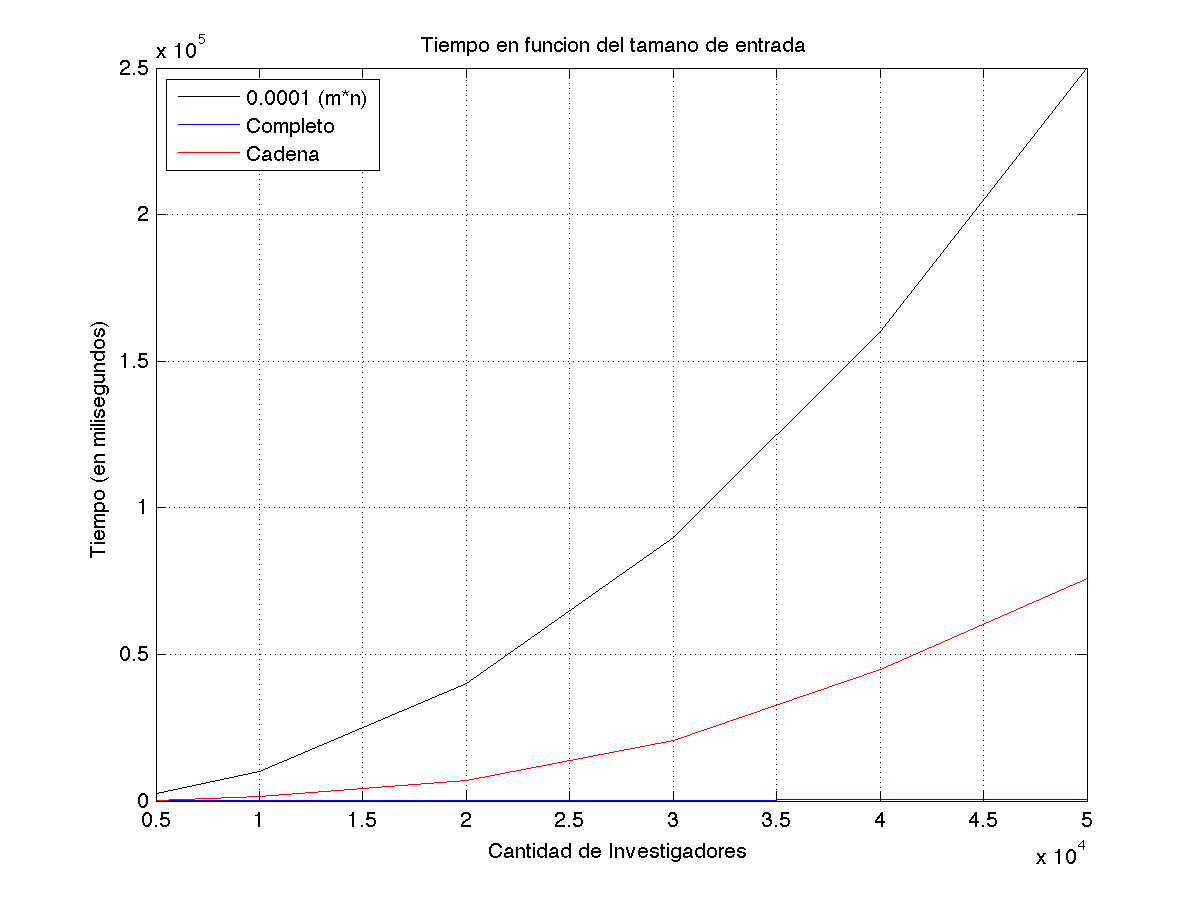
\includegraphics[width=400px]{./figs/cotaComparacion.png}
\end{figure}

En estas dos experimentaciones, lo que se utiliza como entrada es la cuenta $m*n$, siendo $m$ la cantidad de amistades y $n$ la cantidad de investigadores. Se ve claramente como la curva $m*n$ multiplicada por una constante (en este caso en particular, $10^{-3}$) sobrepasa a ambas curvas en todo momento, evidenciando el cumplimiento de la cota de complejidad propuesta por la cátedra.

Cabe destacar que en el caso del grafo completo los tiempos son mucho más rápidos que los mostrados por la cota, e incluso por el caso del grafo cadena, y por eso parece ser una línea recta pegada al eje (\textit{Aclaración: recomendamos verlo en el informe en formato digital, ya que es probable que en la versión impresa no se llegue a distinguir}). Los valores graficados en el grafo completo son:

\begin{center}
\begin{tabular}{|c|c|}\hline
	\textbf{Cantidad de Investigadores}	&	\textbf{Tiempo (en ms)}	\\ \hline
	5.000	&	27	\\ \hline
	10.000	&	48	\\ \hline
	20.000	&	127	\\ \hline
	30.000	&	253	\\ \hline
	40.000	&	370	\\ \hline
	50.000	&	551	\\ \hline
\end{tabular}
\end{center}

Este comportamiento se debe a que escencialmente el problema se resuelve en una sola pasada por las amistades del primer investigador, ya que lo primero que se hace es clasificar como \textit{``encontrado''} al primer investigador, clasificar a todos sus amigos (por ser un grafo completo, se recorre a todos los investigadores restantes) asignándoles también el estado \textit{``encontrado''}, seteando por último, al primer investigador como \textit{``visitado''}. Al ver que los amigos de todos los demás tienen como estado \textit{``encontrado''}, al pasar por ellos no se hace nada más que setear a cada uno como \textit{``visitado''}, ya que nadie tiene amigos que no hayan sido visitados en la primera pasada, finalizando rápidamente el algoritmo.

Debemos hacer una última observación sobre este gráfico, aclarando que en el eje $x$ se muestra la progresión en la cantidad de investigadores, en lugar de hacerlo en el producto de $m*n$, ya que se puede calcular fácilmente la cantidad de amistades con las cuentas que brindamos en cada caso, y además el gráfico queda más claro de esta forma que con los números del producto de $m$ y $n$, que son los siguientes:

\begin{center}
\begin{tabular}{|c|r|r|}
  \hline
 \textbf{Tamaño de entrada} & \textbf{m*n Cadena} & \textbf{m*n Completo}   \\
  \hline
  5.000	&	9.999	&	12.502.500 \\
  \hline
  10.000	&	19.999	&	50.005.000\\
  \hline
  20.000	&	39.999	&	200.010.000\\
  \hline
  30.000	&	49.999	&	450.015.000\\
  \hline
  40.000	&	79.999	&	800.020.000\\
  \hline
  50.000	&	99.999	&	1.250.025.000\\
  \hline
\end{tabular}
\end{center}

Además, realizamos un test que es similar al de Cadena pero con una única diferencia: la cadena se encuentra partida en alguna parte. A este caso lo denominamos ``Cadena No Conexos''. El mismo es un sub-caso del caso Cadena, con la particularidad de que del investigador $i_0$ al $i_n$ es un grafo cadena, y del $i_m$ en adelante también, pero $i_n$ no es amigo de $i_m$.
De forma similar al caso de Cadena, al representar esta red de amistades con un grafo, se nos generan dos caminos simples donde cada uno conecta a todo par de investigadores dentro de un subconjunto de investigadores $I_1 \subset I $ y lo mismo con un subconjunto $I_2$, con $I_1 \cap I_2 = \emptyset $ y nuevamente, cada investigador que no está en el borde de su respectivo subconjunto contenedor, tendrá 2 amigos directos. La cantidad de amistades en este caso es una menos que en el caso Cadena, por ende, hay
\Gather{(k - 1) -1 = k - 2\textnormal{ amistades.}}
\clearpage
\begin{figure}[h]
	\centering
	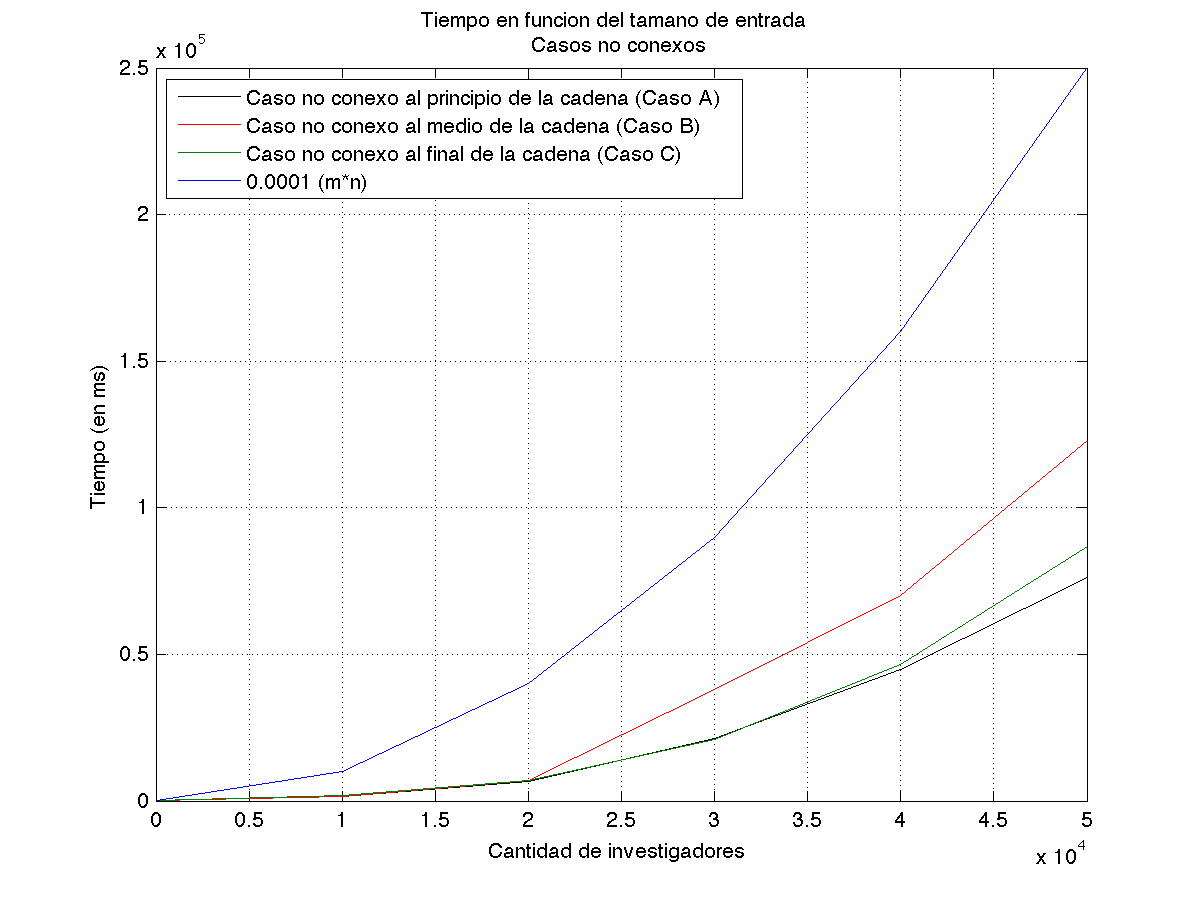
\includegraphics[width=400px]{./figs/noConexo.png}
\end{figure}

En este gráfico representamos 3 casos de esta clase de test. 
\begin{itemize}
	\item Un caso A para una cadena de amistades  partida al principio,  una distancia de 2 investigadores del investigador fuente, es decir, a distancia $2$ del mismo.
	\item Un caso B para una cadena de amistades partida al medio del camino simple que existía entre el investigador fuente y el destino antes de que se ``partiera" la cadena, es decir el corte se realiza en la amistad a distancia $k/2$ del investigador fuente.
	\item Un caso C para una cadena de amistades partida a distancia 2 del investigador destino, es decir en la amistad a distancia $k-2$ del investigador fuente
\end{itemize}

Al igual que con el caso Cadena, se ve claramente el cumplimiento de la cota de complejidad propuesta por la cátedra. Lo que nos llama la atención es el hecho de que el caso B posee una complejidad temporal ampliamente mayor a los otros 2 casos. De hecho, pensamos que el caso C tomaría un tiempo mayor, ya que establecimos inicialmente una relación entre la ubicación del corte con la complejidad temporal, mientras más cercano estuviera el corte del investigador fuente, menos complejidad tomaría. Claramente esta hipótesis se ve refutada con el caso C. Lo que sí es evidente es que el caso A tiene una complejidad menor que los otros dos casos.

\subsubsection{Grafos Random en las Amistades}
El programa que genera un grafo random sobre una cantidad de investigadores fija, toma como parámetro de entrada, la cantidad de investigadores $k$ que tendrá el mismo. Una vez que se tiene dicho parámetro, se genera un archivo que luego se traduce en un grafo en el cual hay $k$ investigadores distintos, y 
para todo investigador $i$ existe algún investigador $j$ tal que $i$ es amigo de $j$ . 

En principio no sabemos cuántas amistades serán en total, pero si sabemos que el máximo de amistades es $\frac{k.(k+1)}{2}$ pues el si todos son amigos de todos es el caso ya mencionado del Grafo Completo. Entonces, el total de amistades está acotado superiormente por  $\frac{k.(k+1)}{2}$.

\begin{figure}[h]
	\centering
	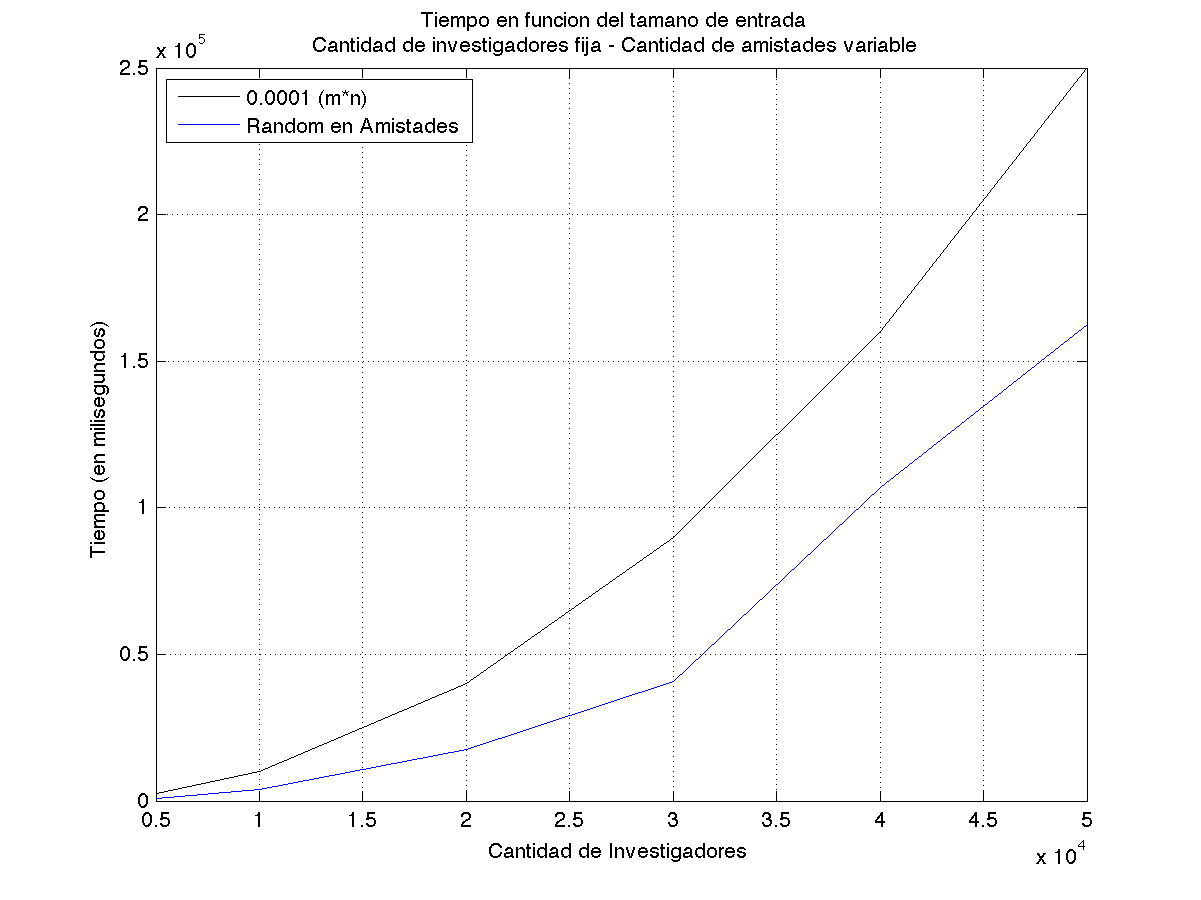
\includegraphics[width=350px]{./figs/cotaInvestigadores.png}
\end{figure}

En esta experimentación volvemos a utilizar la cantidad de investigadores que sabemos que tiene el grafo para realizar el gráfico, ya que la cantidad de amistades se puede acotar pero no se puede saber con certeza, debido a la naturaleza del test.

\subsubsection{Grafos Random en los Investigadores}
El programa que genera un grafo random sobre una cantidad de amistades fija, toma como parámetro de entrada, la cantidad de amistades $n$ que tendrá el mismo. Una vez que se tiene dicho parámetro, se genera un archivo que luego se traduce en un grafo en el cual hay $n$ amistades. 

En principio no sabemos cuántos investigadores serán en total, pero si sabemos que la cantidad de amistades es $n$. No existen investigadores en el sistema que no tengan ningún amigo. Si tenemos en cuenta el caso en el que cada uno tiene la mínima cantidad posible de amigos ($i$ tiene como único amigo a $j$ y viceversa), entonces tendremos $2.n$ investigadores, y para toda amistad $a_1$ no existe una amistad $a_2 \neq a_1$ tal que algún investigador contenido en la amistad $a_1$ no está en $a_2$. Entonces el total de investigadores está acotado superiormente por $2.n$.


\begin{figure}[h]
	\centering
	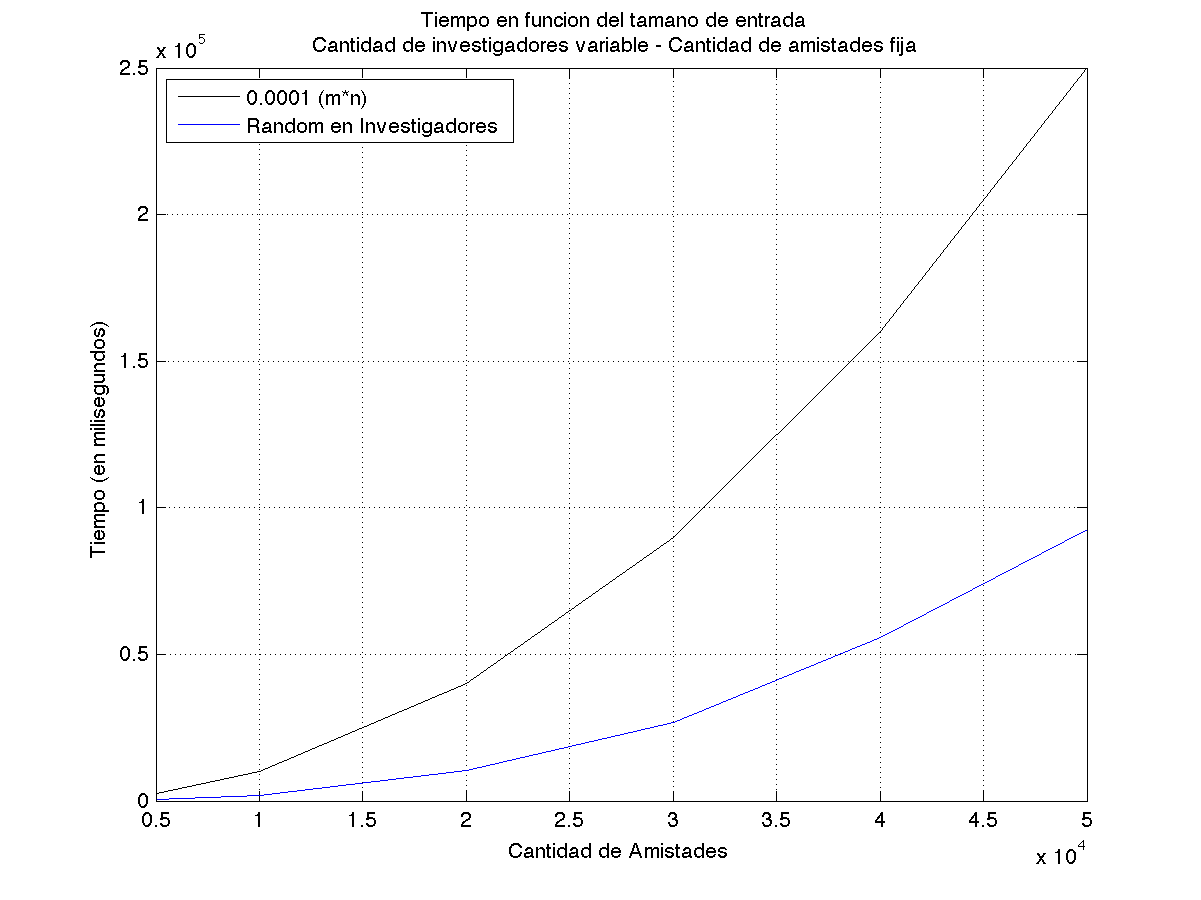
\includegraphics[width=350px]{./figs/cotaAmistades.png}
\end{figure}

A diferencia de los grafos anteriores, en este se utiliza como parámetro de entrada la cantidad de amistades que deseamos que haya en el mismo (por eso no se puede comparar directamente con el resto de los gráficos). Lo que queda claro tanto en este random, como en el anterior, es que ambos cumplen la complejidad requerida. Además, lo que se puede apreciar es que ambos casos tardan más en ser resueltos que los del tipo completo o cadena (pues son los grafos -dentro de los testeados por nosotros- más complejos de resolver para nuestro algoritmo en particular).

%\subsubsection{Grafo Cadena Partida}
%El programa que genera un grafo cadena partida toma como parámetro de entrada, la cantidad de investigadores $k$ que tendrá el mismo. Una vez que se tiene dicho parámetro, se genera un archivo que luego se traduce en un grafo en el cual hay $k$ investigadores distintos, y para todo $i_n, i_m$ con $1 \leq n,m \leq k$ tales que $i_n + 1 = i_m$, $i_n$ e $i_m$ son amigos (es decir, todos tienen como amigo al anterior y al siguiente de la cadena, exceptuando los que se encuentran en los bordes) o $i_n$ no es amigo de $i_m$ y $i_n$ es amigo de $i_{n-1}$ y $i_m$ es amigo de $i_{m+1}$.
%
%Al representar esta red de amistades con un grafo, se nos generan dos caminos simples donde cada uno conecta a todo par de investigadores dentro de un subconjunto de investigadores $I_1 \subset I $ y lo mismo con un subconjunto $I_2$, con $I_1 \cap I_2 = \emptyset $ y donde cada investigador tendrá 2 amigos directos (exceptuando el primero y el último de cada subconjunto, que tienen solamente 1 amigo). Es por esto que el total de amistades será 
%\Gather{(\displaystyle{\sum_{i=2}^{j-1}{2} + \sum_{i=j+2}^{k-1}{2}) + 2 + 2 = 2.(j-1-2) + 2.(k-1-j-2)+ 4 = 2.j-6+2.k-2.j-6+4= 2.k-8}}
%si las contamos de manera aislada, pero estaríamos contando a la mayoría dos veces. Por este motivo, dicha cantidad debe ser dividida por 2 para conseguir la cantidad real de amistades del grafo, que es 
%\Gather{\frac {2.k-8}{2} = k-4}
%
%\begin{figure}[h]
%	\centering
%	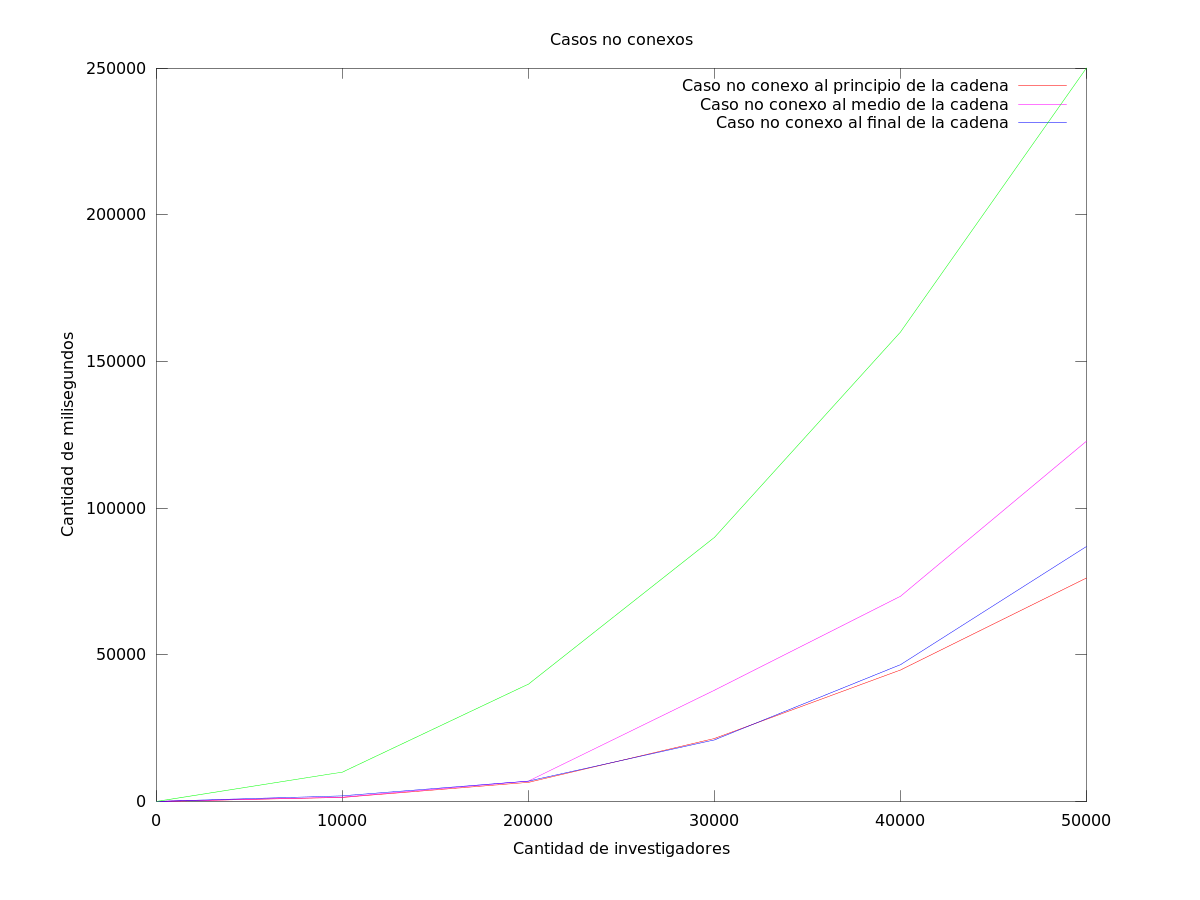
\includegraphics[width=400px]{./figs/comparacionCasos.png}
%\end{figure}
%
%En este gráfico representamos 3 casos de esta clase de test. 
%\begin{itemize}
%	\item Un caso A para una cadena de amistades  partida al principio,  una distancia de 2 investigadores del investigador fuente, es decir, a distancia $2$ del mismo.
%	\item Un caso B para una cadena de amistades partida al medio del camino simple que existía entre el investigador fuente y el destino antes de que se "partiera" la cadena, es decir el corte se realiza en la amistad a distancia $k/2$ del investigador fuente.
%	\item Un caso C para una cadena de amistades partida a distancia 2 del investigador destino, es decir en la amistad a distancia $k-2$ del investigador fuente
%\end{itemize}
%
%En esta experimentación, lo que se utiliza como entrada es la cuenta $m*n$, siendo $m$ la cantidad de amistades y $n$ la cantidad de investigadores. Se ve claramente como la curva $m*n$ multiplicada por una constante (en este caso en particular, $10^{-3}$) sobrepasa a las 3 curvas en todo momento y tienen una pendiente similar, evidenciando el cumplimiento de la cota de complejidad propuesta por la cátedra.
%
%Lo que nos llama la atención es el hecho de que el caso B toma una complejidad temporal ampliamente mayor a los otros 2 casos. De hecho, pensamos que el caso C tomaría un tiempo mayor, ya que establecimos inicialmente una relación entre la ubicación del corte con la complejidad temporal, mientras más cercano estuviera el corte del investigador fuente, menos complejidad tomaría. Claramente esta hipótesis se ve refutada con el caso C. Lo que sí es evidente es que el caso A toma una complejidad menor que los otros dos.

%\indent Al igual que para el ejercicio 1, corrimos los casos de test 1000 veces
%para poder obtener un tiempo que sea significativo de mostrar en $ms$. A
%continuación presentamos el caso de prueba all vs all:
%
%\begin{figure}[h]
%\centering                                                       
%        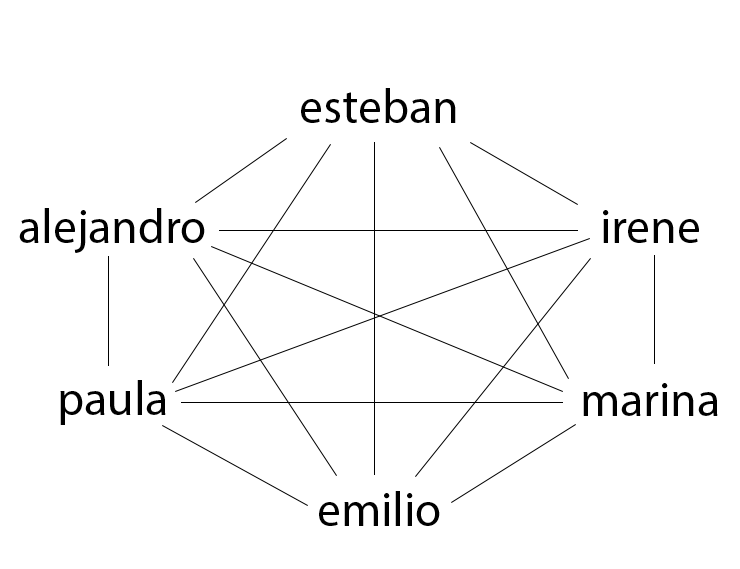
\includegraphics[width=130pt]{./figs/todosVStodos.png}
%	\caption{Aquí se representa el grafo correspondiente al caso de test
%'AllvsAll'}
%	\label{fig:tvst}
%\end{figure}
%\indent Teniendo en cuenta este caso y los proporcionados por la cátedra,
%realizamos las corridas para evaluar su tiempo de ejecución.
%\begin{center}
%\begin{tabular}{|c|c|}
%  \hline
%  Caso de test & Tiempo de ejecución de 1000 corridas $(ms)$   \\
%  \hline
%  1        &  11   \\
%  \hline
%  2        & 213\\
%  \hline
%  3        & 370      \\
%  \hline
%  4        & 350        \\
%  \hline
%  5  	   & 384    \\
%  \hline
%  6        & 665\\
%  \hline
%   7 	& 628        \\
%  \hline  
%  all vs all 	& 152        \\
%  \hline
%\end{tabular}
%\end{center}
%
%\indent En la tabla los casos 1-7 representan los casos del archivo
%$tp1ej2.in$.\\
%\indent Podemos observar claramente como influye que la complejidad es
%\Gather{O(k)*O(a) = O(cantidad\ de\ investigadores)*O(cantidad\ de\ amistades)}
%en el tiempo de ejecución. \\
%\indent Esto lo podemos ver como un claro ejemplo en el caso 1 adonde al no
%tener amistades tenemos un tiempo de muy bajo de solo $11ms$.
%En cambio en los casos que mas investigadores y amistades tienen (casos 6 y 7)
%son los que mas tardan si los comparamos con los casos 1-5 que no tienen tantos
%investigadores/relaciones.
